%===================================================================================================
% Embedding Concepts for Statistical Research
% LaTeX Beamer presentation
%===================================================================================================

\documentclass[aspectratio=169]{beamer}

%===================================================================================================
% Theme and packages
%===================================================================================================

\usetheme{Madrid}
\usecolortheme{default}
\setbeamertemplate{navigation symbols}{}
\setbeamertemplate{footline}[frame number]

\usepackage[utf8]{inputenc}
\usepackage[T1]{fontenc}
\usepackage{lmodern}
\usepackage{amsmath, amsfonts, amssymb}
\usepackage{booktabs}
\usepackage{array}
\usepackage{tikz}
\usetikzlibrary{arrows.meta, positioning, shapes.geometric, calc}
\usepackage{xcolor}
\usepackage{tcolorbox}
\usepackage{hyperref}

%===================================================================================================
% Colors and commands
%===================================================================================================

\definecolor{deepblue}{RGB}{30,70,130}
\definecolor{softblue}{RGB}{230,240,255}
\definecolor{darkgreen}{RGB}{20,110,70}
\definecolor{softgreen}{RGB}{230,247,238}
\definecolor{darkred}{RGB}{155,45,45}
\definecolor{softred}{RGB}{252,235,235}
\definecolor{darkgray}{RGB}{65,65,65}
\definecolor{lightgray}{RGB}{245,245,245}
\definecolor{orangeaccent}{RGB}{220,120,35}

\setbeamercolor{title}{fg=deepblue}
\setbeamercolor{frametitle}{fg=deepblue}
\setbeamercolor{structure}{fg=deepblue}

\newcommand{\R}{\mathbb{R}}
\newcommand{\E}{\mathbb{E}}
\newcommand{\Var}{\operatorname{Var}}
\newcommand{\Cov}{\operatorname{Cov}}
\newcommand{\argmin}{\operatorname*{arg\,min}}
\newcommand{\vect}[1]{\boldsymbol{#1}}

\newtcolorbox{bluebox}{colback=softblue,colframe=deepblue,boxrule=0.7pt,arc=2mm,left=1.5mm,right=1.5mm,top=1mm,bottom=1mm}
\newtcolorbox{greenbox}{colback=softgreen,colframe=darkgreen,boxrule=0.7pt,arc=2mm,left=1.5mm,right=1.5mm,top=1mm,bottom=1mm}
\newtcolorbox{redbox}{colback=softred,colframe=darkred,boxrule=0.7pt,arc=2mm,left=1.5mm,right=1.5mm,top=1mm,bottom=1mm}

%===================================================================================================
% Title
%===================================================================================================

\title[Embeddings for Statistical Research]{Embeddings for Statistical Research\\\large From Raw Objects to Quantitative Features}
\author{Internal Research Seminar}
\institute{Prepared for an academic statistics audience}
\date{\today}

%===================================================================================================
% Document
%===================================================================================================

\begin{document}

%---------------------------------------------------------------------------------------------------
\begin{frame}
  \titlepage
\end{frame}

%---------------------------------------------------------------------------------------------------
\begin{frame}{Seminar objective}
\large
The goal is to make the concept of an \textbf{embedding} precise enough for statistical researchers.

\vspace{0.3cm}

\begin{bluebox}
An embedding is a map that converts an object such as a word, a document, an image, a graph, a molecule, or a financial news article into a numerical vector that can be used in statistical models.
\end{bluebox}

\vspace{0.3cm}

By the end of the seminar, we should understand:
\begin{itemize}
  \item what embeddings are from a statistical point of view;
  \item how text embeddings differ from bag-of-words and dictionaries;
  \item why LLM embeddings can be used as covariates in regression;
  \item what methodological risks they introduce.
\end{itemize}
\end{frame}

%---------------------------------------------------------------------------------------------------
\begin{frame}{Why this matters for our research program}
\large
Modern empirical research increasingly uses data that are not naturally tabular:

\vspace{0.2cm}

\begin{itemize}
  \item financial news, analyst reports, filings, earnings call transcripts;
  \item scientific papers, patents, legal documents;
  \item product descriptions, firm descriptions, customer feedback;
  \item code, logs, graphs, images, and multimodal records.
\end{itemize}

\vspace{0.25cm}

\begin{greenbox}
Embeddings are the bridge between \textbf{unstructured information} and \textbf{statistical modeling}.
\end{greenbox}

\vspace{0.2cm}

They allow us to ask familiar statistical questions on unfamiliar objects.
\end{frame}

%---------------------------------------------------------------------------------------------------
\begin{frame}{The statistical abstraction}
\large
Let \(\mathcal{X}\) be a space of objects. Examples:

\vspace{0.2cm}

\begin{itemize}
  \item \(\mathcal{X}\): all English financial news articles;
  \item \(\mathcal{X}\): all firm descriptions;
  \item \(\mathcal{X}\): all hyperparameter configurations;
  \item \(\mathcal{X}\): all graphs representing supply chains.
\end{itemize}

\vspace{0.3cm}

An embedding is a feature map

\[
\phi : \mathcal{X} \longrightarrow \R^d,
\]

where \(\phi(x)\) is a vector representation of object \(x\), and \(d\) is the embedding dimension.
\end{frame}

%---------------------------------------------------------------------------------------------------
\begin{frame}{Embeddings as feature maps}
\large
Once \(x\) has been mapped to \(\phi(x)\), we can use standard statistical models:

\[
Y = g\big(\phi(X)\big) + \varepsilon.
\]

\vspace{0.2cm}

Here:
\begin{itemize}
  \item \(X \in \mathcal{X}\) is the original object;
  \item \(Y \in \R\) is the target variable;
  \item \(\phi(X) \in \R^d\) is the embedding;
  \item \(g : \R^d \to \R\) is a regression function;
  \item \(\varepsilon\) is an error term.
\end{itemize}

\vspace{0.2cm}

\begin{bluebox}
The embedding is not the model. It is the representation on which the model operates.
\end{bluebox}
\end{frame}

%---------------------------------------------------------------------------------------------------
\begin{frame}{A familiar example: categorical variables}
\large
Statisticians have used embeddings for a long time, even without calling them embeddings.

\vspace{0.2cm}

Suppose a variable \(C\) takes values in three categories:

\[
C \in \{\text{Technology},\text{Banking},\text{Energy}\}.
\]

A one-hot encoding is an embedding:

\[
\phi(\text{Technology})=(1,0,0), \quad
\phi(\text{Banking})=(0,1,0), \quad
\phi(\text{Energy})=(0,0,1).
\]

\vspace{0.2cm}

It maps a non-numeric object into a vector space.
\end{frame}

%---------------------------------------------------------------------------------------------------
\begin{frame}{From sparse to dense representations}
\large
Classical encodings are often \textbf{sparse} and high-dimensional.

\vspace{0.25cm}

\begin{columns}[T]
\begin{column}{0.48\textwidth}
\begin{bluebox}
\textbf{Sparse representation}
\begin{itemize}
  \item one-hot vectors;
  \item bag-of-words counts;
  \item thousands of zero entries;
  \item weak notion of similarity.
\end{itemize}
\end{bluebox}
\end{column}
\begin{column}{0.48\textwidth}
\begin{greenbox}
\textbf{Dense representation}
\begin{itemize}
  \item learned numerical vectors;
  \item most coordinates nonzero;
  \item compact semantic information;
  \item meaningful geometry.
\end{itemize}
\end{greenbox}
\end{column}
\end{columns}

\vspace{0.4cm}

Modern text embeddings are dense vector representations learned from large corpora.
\end{frame}

%---------------------------------------------------------------------------------------------------
\begin{frame}{The key idea: geometry}
\large
An embedding does more than assign numbers. It creates a geometry.

\vspace{0.3cm}

\begin{center}
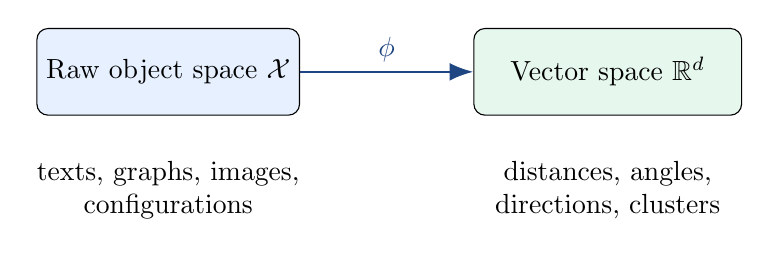
\begin{tikzpicture}[scale=0.92]
  \node[draw, rounded corners, fill=softblue, minimum width=3.2cm, minimum height=1.1cm] (raw) {Raw object space \(\mathcal{X}\)};
  \node[draw, rounded corners, fill=softgreen, minimum width=3.4cm, minimum height=1.1cm, right=2.2cm of raw] (vec) {Vector space \(\R^d\)};
  \draw[-{Latex[length=3mm]}, thick, deepblue] (raw) -- node[above] {\(\phi\)} (vec);
  \node[below=0.45cm of raw, align=center] {texts, graphs, images,\\configurations};
  \node[below=0.45cm of vec, align=center] {distances, angles,\\directions, clusters};
\end{tikzpicture}
\end{center}

\vspace{0.3cm}

A good embedding should place \textbf{similar objects} near each other and should organize variation in useful directions.
\end{frame}

%---------------------------------------------------------------------------------------------------
\begin{frame}{Similarity in embedding space}
\large
Given two objects \(x_a,x_b \in \mathcal{X}\), their embeddings are

\[
\vect{z}_a = \phi(x_a), \qquad \vect{z}_b = \phi(x_b),
\]

where \(\vect{z}_a,\vect{z}_b \in \R^d\).

\vspace{0.3cm}

Common similarity measures include:

\[
\text{Euclidean distance: } \|\vect{z}_a-\vect{z}_b\|_2,
\]

\[
\text{Cosine similarity: }
\frac{\vect{z}_a'\vect{z}_b}{\|\vect{z}_a\|_2\|\vect{z}_b\|_2}.
\]

\vspace{0.2cm}

These are not merely technical details: they define what the model treats as close, far, similar, or different.
\end{frame}

%---------------------------------------------------------------------------------------------------
\begin{frame}{A statistical view of text}
\large
Text is hard for standard statistics because it is:

\vspace{0.15cm}

\begin{itemize}
  \item variable-length;
  \item high-dimensional;
  \item ordered;
  \item context-dependent;
  \item ambiguous;
  \item rich in latent structure.
\end{itemize}

\vspace{0.3cm}

A sentence is not a vector in a natural way. An embedding model defines a map:

\[
\phi(\text{document}) \in \R^d.
\]

\vspace{0.15cm}

After this map is defined, text can enter a regression, classification, clustering, or portfolio-construction model.
\end{frame}

%---------------------------------------------------------------------------------------------------
\begin{frame}{Bag-of-words: the classical baseline}
\large
The bag-of-words representation maps a document to word counts:

\[
\phi_{\text{BoW}}(x) = (c_1(x),c_2(x),\ldots,c_V(x)),
\]

where:
\begin{itemize}
  \item \(V\) is the vocabulary size;
  \item \(c_j(x)\) is the count of word \(j\) in document \(x\).
\end{itemize}

\vspace{0.3cm}

\begin{redbox}
Bag-of-words ignores word order and context. The phrases \textit{``losses increased''} and \textit{``losses were erased''} may look too similar.
\end{redbox}
\end{frame}

%---------------------------------------------------------------------------------------------------
\begin{frame}{Dictionary sentiment as a low-dimensional embedding}
\large
A finance dictionary method can be written as

\[
\phi_{\text{dict}}(x) = s(x),
\]

where \(s(x) \in \R\) is a scalar sentiment score.

\vspace{0.25cm}

For example,

\[
s(x) = \frac{\#\text{positive words}-\#\text{negative words}}{\#\text{total words}}.
\]

\vspace{0.3cm}

This is an embedding into \(\R^1\). It is simple and interpretable, but it compresses the document aggressively.

\vspace{0.2cm}

\begin{bluebox}
The statistical question is a bias-variance trade-off: scalar sentiment is low variance but high bias; LLM embeddings are richer but higher-dimensional.
\end{bluebox}
\end{frame}

%---------------------------------------------------------------------------------------------------
\begin{frame}{Distributional semantics}
\large
Word embeddings are based on a simple principle:

\vspace{0.25cm}

\begin{greenbox}
Words that appear in similar contexts tend to have related meanings.
\end{greenbox}

\vspace{0.35cm}

A model learns a map

\[
\phi_{\text{word}} : \mathcal{V} \to \R^d,
\]

where \(\mathcal{V}\) is a vocabulary and \(\phi_{\text{word}}(w)\) is the vector representation of word \(w\).

\vspace{0.25cm}

Classic examples include Word2Vec, GloVe, and fastText.
\end{frame}

%---------------------------------------------------------------------------------------------------
\begin{frame}{Static word embeddings}
\large
In static word embeddings, each word has one vector:

\[
\phi_{\text{word}}(\text{``bank''}) = \vect{v}_{\text{bank}}.
\]

\vspace{0.25cm}

This is useful but limited:

\begin{itemize}
  \item \textit{bank} as a financial institution;
  \item \textit{bank} as the side of a river.
\end{itemize}

\vspace{0.25cm}

Both meanings receive the same vector.

\vspace{0.25cm}

\begin{redbox}
Static embeddings learn average meaning, not context-specific meaning.
\end{redbox}
\end{frame}

%---------------------------------------------------------------------------------------------------
\begin{frame}{Contextual embeddings}
\large
Modern language models produce context-dependent embeddings.

\vspace{0.2cm}

The same token can have different vectors in different sentences:

\[
\phi(\text{``bank''} \mid \text{``central bank raised rates''})
\]

\[
\phi(\text{``bank''} \mid \text{``river bank collapsed''}).
\]

\vspace{0.3cm}

The embedding depends on the surrounding text.

\vspace{0.2cm}

\begin{bluebox}
This is why Transformer-based embeddings are more informative than word counts: they encode context, word order, and long-range dependencies.
\end{bluebox}
\end{frame}

%---------------------------------------------------------------------------------------------------
\begin{frame}{The Transformer embedding pipeline}
\large
A simplified document embedding pipeline is:

\vspace{0.3cm}

\begin{center}
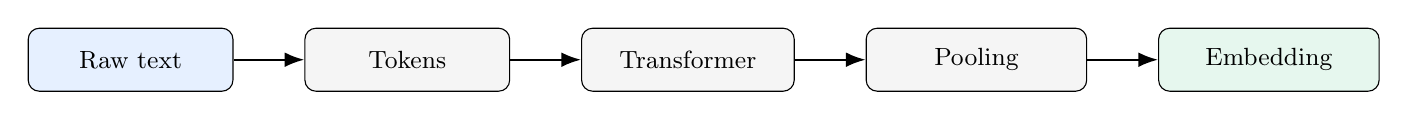
\begin{tikzpicture}[node distance=1.1cm, every node/.style={font=\small}]
  \node[draw, rounded corners, fill=softblue, minimum width=2.6cm, minimum height=0.8cm] (text) {Raw text};
  \node[draw, rounded corners, fill=lightgray, minimum width=2.6cm, minimum height=0.8cm, right=0.9cm of text] (tok) {Tokens};
  \node[draw, rounded corners, fill=lightgray, minimum width=2.7cm, minimum height=0.8cm, right=0.9cm of tok] (tr) {Transformer};
  \node[draw, rounded corners, fill=lightgray, minimum width=2.8cm, minimum height=0.8cm, right=0.9cm of tr] (pool) {Pooling};
  \node[draw, rounded corners, fill=softgreen, minimum width=2.8cm, minimum height=0.8cm, right=0.9cm of pool] (emb) {Embedding};
  \draw[-{Latex[length=2.5mm]}, thick] (text) -- (tok);
  \draw[-{Latex[length=2.5mm]}, thick] (tok) -- (tr);
  \draw[-{Latex[length=2.5mm]}, thick] (tr) -- (pool);
  \draw[-{Latex[length=2.5mm]}, thick] (pool) -- (emb);
\end{tikzpicture}
\end{center}

\vspace{0.4cm}

If the document has \(L\) tokens and token embeddings have dimension \(d\), the Transformer returns approximately an \(L \times d\) matrix. Pooling converts it into one vector in \(\R^d\).
\end{frame}

%---------------------------------------------------------------------------------------------------
\begin{frame}{Pooling: from tokens to documents}
\large
Let a document be tokenized into \(L\) tokens.

\vspace{0.15cm}

Let \(\vect{h}_\ell \in \R^d\) be the contextual embedding of token \(\ell\), for \(\ell=1,\ldots,L\).

\vspace{0.25cm}

A simple document embedding is mean pooling:

\[
\phi(x) = \frac{1}{L}\sum_{\ell=1}^{L}\vect{h}_\ell.
\]

\vspace{0.25cm}

Here:
\begin{itemize}
  \item \(x\) is the document;
  \item \(L\) is the number of tokens;
  \item \(\vect{h}_\ell\) is the vector for token \(\ell\);
  \item \(\phi(x)\) is the document-level embedding.
\end{itemize}
\end{frame}

%---------------------------------------------------------------------------------------------------
\begin{frame}{Frozen embeddings and downstream models}
\large
In many empirical applications, the LLM is not re-trained.

\vspace{0.3cm}

\begin{center}
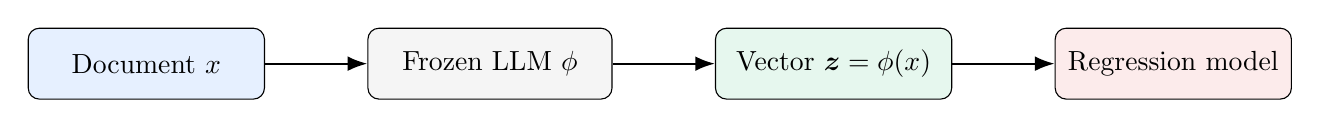
\begin{tikzpicture}[node distance=1.3cm]
  \node[draw, rounded corners, fill=softblue, minimum width=3.0cm, minimum height=0.9cm] (doc) {Document \(x\)};
  \node[draw, rounded corners, fill=lightgray, minimum width=3.1cm, minimum height=0.9cm, right=1.3cm of doc] (llm) {Frozen LLM \(\phi\)};
  \node[draw, rounded corners, fill=softgreen, minimum width=3.0cm, minimum height=0.9cm, right=1.3cm of llm] (z) {Vector \(\vect{z}=\phi(x)\)};
  \node[draw, rounded corners, fill=softred, minimum width=3.0cm, minimum height=0.9cm, right=1.3cm of z] (model) {Regression model};
  \draw[-{Latex[length=2.5mm]}, thick] (doc) -- (llm);
  \draw[-{Latex[length=2.5mm]}, thick] (llm) -- (z);
  \draw[-{Latex[length=2.5mm]}, thick] (z) -- (model);
\end{tikzpicture}
\end{center}

\vspace{0.4cm}

Only the downstream statistical model is fitted to the research target \(Y\).

\vspace{0.2cm}

\begin{bluebox}
The LLM supplies a representation; the researcher estimates the predictive relationship.
\end{bluebox}
\end{frame}

%---------------------------------------------------------------------------------------------------
\begin{frame}{Embeddings in regression}
\large
A standard embedding-based regression is

\[
Y_i = \alpha + \phi(X_i)'\vect{\beta} + \varepsilon_i,
\]

where:
\begin{itemize}
  \item \(X_i\) is the original object for observation \(i\);
  \item \(Y_i\) is the target variable;
  \item \(\phi(X_i) \in \R^d\) is the embedding;
  \item \(\vect{\beta} \in \R^d\) is the coefficient vector;
  \item \(\varepsilon_i\) is the residual error.
\end{itemize}

\vspace{0.2cm}

When \(d\) is large, regularization is usually necessary.
\end{frame}

%---------------------------------------------------------------------------------------------------
\begin{frame}{Regularization is not optional}
\large
For high-dimensional embeddings, a common estimator is ridge regression:

\[
\widehat{\vect{\beta}}
=
\argmin_{\vect{\beta} \in \R^d}
\sum_{i=1}^{n}\left(Y_i-\alpha-\phi(X_i)'\vect{\beta}\right)^2
+
\lambda\|\vect{\beta}\|_2^2.
\]

\vspace{0.2cm}

Here:
\begin{itemize}
  \item \(n\) is the number of observations;
  \item \(d\) is the embedding dimension;
  \item \(\lambda \geq 0\) controls shrinkage;
  \item \(\|\vect{\beta}\|_2^2=\sum_{j=1}^{d}\beta_j^2\).
\end{itemize}

\vspace{0.2cm}

\begin{greenbox}
Ridge regression is a natural baseline because embeddings are dense, correlated, and high-dimensional.
\end{greenbox}
\end{frame}

%---------------------------------------------------------------------------------------------------
\begin{frame}{Embedding dimensions are not ordinary variables}
\large
A crucial warning for statistical interpretation:

\vspace{0.3cm}

\begin{redbox}
The coordinates of an LLM embedding usually do not have direct human-readable meaning.
\end{redbox}

\vspace{0.3cm}

Therefore, in a model such as

\[
Y_i = \alpha + \sum_{j=1}^{d}\beta_j\phi_j(X_i)+\varepsilon_i,
\]

we should not interpret \(\beta_j\) as the coefficient of a clearly named economic variable.

\vspace{0.25cm}

It is often better to interpret \(\vect{\beta}\) as a \textbf{direction} in embedding space associated with the target.
\end{frame}

%---------------------------------------------------------------------------------------------------
\begin{frame}{A useful analogy: latent factors}
\large
Embeddings resemble latent factor representations.

\vspace{0.2cm}

A factor model writes

\[
\vect{x}_i \approx \vect{\Lambda}\vect{f}_i + \vect{u}_i,
\]

where \(\vect{f}_i\) is a low-dimensional latent representation.

\vspace{0.25cm}

An embedding model writes

\[
\vect{z}_i = \phi(x_i),
\]

where \(\vect{z}_i\) is a learned representation of object \(x_i\).

\vspace{0.25cm}

\begin{bluebox}
Difference: in LLM embeddings, the representation was learned from large external corpora, not necessarily from the dataset used in the downstream regression.
\end{bluebox}
\end{frame}

%---------------------------------------------------------------------------------------------------
\begin{frame}{A useful analogy: kernels}
\large
Kernel methods use a feature map, often implicitly:

\[
k(x_a,x_b)=\langle \phi(x_a),\phi(x_b)\rangle.
\]

\vspace{0.25cm}

Here:
\begin{itemize}
  \item \(k(x_a,x_b)\) is a kernel similarity;
  \item \(\phi(x_a)\) and \(\phi(x_b)\) are feature representations;
  \item \(\langle \cdot,\cdot \rangle\) denotes an inner product.
\end{itemize}

\vspace{0.25cm}

LLM embeddings make the feature map explicit:

\[
x \mapsto \phi_{\text{LLM}}(x) \in \R^d.
\]

\vspace{0.15cm}

This connects language models with familiar ideas from nonparametric statistics.
\end{frame}

%---------------------------------------------------------------------------------------------------
\begin{frame}{Why embeddings can help regression}
\large
An embedding may help if it makes the target function easier to approximate.

\vspace{0.25cm}

Suppose

\[
Y = f(X)+\varepsilon.
\]

After embedding, we model

\[
Y = g(\phi(X))+\varepsilon.
\]

\vspace{0.25cm}

The hope is that \(g\) is simpler than \(f\) because \(\phi\) has organized the input space in a useful way.

\vspace{0.25cm}

\begin{redbox}
This is not guaranteed. It is an empirical property of the pair \((\phi,f)\), not a universal property of the embedding.
\end{redbox}
\end{frame}

%---------------------------------------------------------------------------------------------------
\begin{frame}{Smoothness and local structure}
\large
A representation is useful for regression when nearby embedded points tend to have similar target values.

\vspace{0.2cm}

For two objects \(x_a,x_b\), define a local ratio:

\[
L(x_a,x_b)
=
\frac{|f(x_a)-f(x_b)|}{\|\phi(x_a)-\phi(x_b)\|_2}.
\]

\vspace{0.2cm}

Here:
\begin{itemize}
  \item \(f(x_a),f(x_b)\) are target function values;
  \item \(\phi(x_a),\phi(x_b)\) are embeddings;
  \item \(L(x_a,x_b)\) is a local Lipschitz-like factor.
\end{itemize}

\vspace{0.2cm}

Small values suggest that the target varies smoothly in embedding space.
\end{frame}

%---------------------------------------------------------------------------------------------------
\begin{frame}{Important limitation: embeddings do not know the target}
\large
When the LLM is frozen, \(\phi(X)\) depends only on \(X\), not on \(Y\).

\vspace{0.3cm}

\[
X \longrightarrow \phi(X)
\]

is computed before fitting the downstream model.

\vspace{0.25cm}

The target \(Y\) enters only when estimating

\[
Y = g(\phi(X))+\varepsilon.
\]

\vspace{0.3cm}

\begin{bluebox}
Therefore, if an embedding helps prediction, it is because its pre-existing geometry happens to be compatible with the target problem.
\end{bluebox}
\end{frame}

%---------------------------------------------------------------------------------------------------
\begin{frame}{Application example: financial news}
\large
For a financial news article \(x_{i,t}\) about stock \(i\) at time \(t\), compute

\[
\vect{z}_{i,t}=\phi(x_{i,t}) \in \R^d.
\]

Then estimate a predictive model such as

\[
\E(r_{i,t+1}\mid \vect{z}_{i,t}) = \vect{z}_{i,t}'\vect{\beta},
\]

where:
\begin{itemize}
  \item \(r_{i,t+1}\) is the future return of stock \(i\);
  \item \(\vect{z}_{i,t}\) is the news embedding;
  \item \(\vect{\beta}\) is the estimated predictive direction.
\end{itemize}

\vspace{0.2cm}

This is a direct use of embeddings as high-dimensional regressors.
\end{frame}

%---------------------------------------------------------------------------------------------------
\begin{frame}{Raw news embeddings versus news shocks}
\large
In asset pricing, not all news text is truly new information.

\vspace{0.2cm}

Let \(\vect{E}_{i,t}\in\R^d\) be a stock-month news embedding and \(\vect{S}_{i,t}\in\R^p\) be known stock characteristics.

\vspace{0.2cm}

A residualization step can be written as

\[
\vect{E}_{i,t} = \vect{B}'\vect{S}_{i,t}+\vect{\varepsilon}_{i,t}.
\]

Here:
\begin{itemize}
  \item \(\vect{B}\) is a coefficient matrix;
  \item \(\vect{B}'\vect{S}_{i,t}\) is predictable news content;
  \item \(\vect{\varepsilon}_{i,t}\) is the residual news shock.
\end{itemize}

\vspace{0.15cm}

The statistical idea is familiar: separate predictable components from innovations.
\end{frame}

%---------------------------------------------------------------------------------------------------
\begin{frame}{Why statisticians should care}
\large
Embedding-based research raises several statistical questions:

\vspace{0.2cm}

\begin{itemize}
  \item What population object does an embedding represent?
  \item What is the effect of using a pre-trained representation learned from external data?
  \item How should we regularize high-dimensional dense covariates?
  \item How do we interpret coefficients when coordinates are latent?
  \item How do we avoid leakage, look-ahead bias, and benchmark contamination?
  \item How stable are embeddings across model versions and providers?
\end{itemize}

\vspace{0.2cm}

\begin{greenbox}
Embeddings make new data usable, but they also make the measurement process model-dependent.
\end{greenbox}
\end{frame}

%---------------------------------------------------------------------------------------------------
\begin{frame}{Anisotropy and normalization}
\large
LLM embeddings often exhibit \textbf{anisotropy}: many unrelated documents have surprisingly high similarity.

\vspace{0.2cm}

Consequences:
\begin{itemize}
  \item common directions may dominate distances;
  \item raw cosine similarities may be misleading;
  \item downstream regressions may use nuisance variation.
\end{itemize}

\vspace{0.25cm}

Common preprocessing steps include:

\[
\widetilde{z}_{i,j} = \frac{z_{i,j}-\widehat{\mu}_{j}}{\widehat{\sigma}_{j}},
\]

where \(z_{i,j}\) is coordinate \(j\) of embedding \(i\), and \(\widehat{\mu}_{j},\widehat{\sigma}_{j}\) are estimated coordinate-level moments.
\end{frame}

%---------------------------------------------------------------------------------------------------
\begin{frame}{Prediction versus explanation}
\large
Embeddings are extremely useful for prediction, but explanation is harder.

\vspace{0.25cm}

\begin{columns}[T]
\begin{column}{0.48\textwidth}
\begin{greenbox}
\textbf{Prediction}
\begin{itemize}
  \item Does \(\phi(X)\) improve out-of-sample performance?
  \item Does it add incremental information?
  \item Is performance robust through time?
\end{itemize}
\end{greenbox}
\end{column}
\begin{column}{0.48\textwidth}
\begin{redbox}
\textbf{Explanation}
\begin{itemize}
  \item What concepts drive the prediction?
  \item Which semantic themes matter?
  \item Are we measuring causal information or correlation?
\end{itemize}
\end{redbox}
\end{column}
\end{columns}

\vspace{0.25cm}

For explanation, additional tools are needed: clustering, topic models, sparse autoencoders, perturbation tests, or human validation.
\end{frame}

%---------------------------------------------------------------------------------------------------
\begin{frame}{Embedding-based empirical pipeline}
\large
A practical research pipeline is:

\vspace{0.25cm}

\begin{center}
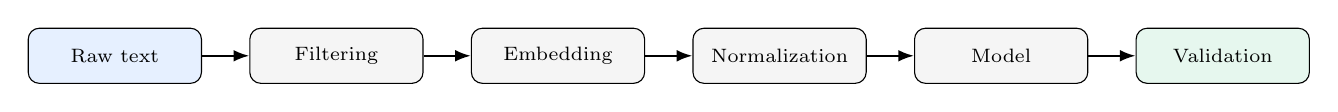
\begin{tikzpicture}[node distance=0.85cm, every node/.style={font=\scriptsize}]
  \node[draw, rounded corners, fill=softblue, minimum width=2.2cm, minimum height=0.7cm] (raw) {Raw text};
  \node[draw, rounded corners, fill=lightgray, minimum width=2.2cm, minimum height=0.7cm, right=0.6cm of raw] (clean) {Filtering};
  \node[draw, rounded corners, fill=lightgray, minimum width=2.2cm, minimum height=0.7cm, right=0.6cm of clean] (emb) {Embedding};
  \node[draw, rounded corners, fill=lightgray, minimum width=2.2cm, minimum height=0.7cm, right=0.6cm of emb] (norm) {Normalization};
  \node[draw, rounded corners, fill=lightgray, minimum width=2.2cm, minimum height=0.7cm, right=0.6cm of norm] (model) {Model};
  \node[draw, rounded corners, fill=softgreen, minimum width=2.2cm, minimum height=0.7cm, right=0.6cm of model] (eval) {Validation};
  \draw[-{Latex[length=2mm]}, thick] (raw) -- (clean);
  \draw[-{Latex[length=2mm]}, thick] (clean) -- (emb);
  \draw[-{Latex[length=2mm]}, thick] (emb) -- (norm);
  \draw[-{Latex[length=2mm]}, thick] (norm) -- (model);
  \draw[-{Latex[length=2mm]}, thick] (model) -- (eval);
\end{tikzpicture}
\end{center}

\vspace{0.3cm}

At each step, statistical choices enter: sampling, time alignment, leakage control, normalization, regularization, and out-of-sample design.
\end{frame}

%---------------------------------------------------------------------------------------------------
\begin{frame}{Design choices that matter}
\large
For empirical work, the following choices are not neutral:

\vspace{0.2cm}

\begin{itemize}
  \item \textbf{Model choice}: BERT, RoBERTa, LLaMA, E5, GPT-style embedding models.
  \item \textbf{Document unit}: headline, full article, summary, paragraph, monthly aggregation.
  \item \textbf{Pooling rule}: mean pooling, special token, last token, learned pooling.
  \item \textbf{Normalization}: raw vectors, z-scores, whitening, demeaning.
  \item \textbf{Timing}: when was the text available relative to the target?
  \item \textbf{Downstream estimator}: ridge, lasso, random forest, neural network, portfolio objective.
\end{itemize}

\vspace{0.15cm}

These choices should be treated as part of the empirical design, not as implementation details.
\end{frame}

%---------------------------------------------------------------------------------------------------
\begin{frame}{Common failure modes}
\large
Embedding-based studies can fail for subtle reasons:

\vspace{0.2cm}

\begin{itemize}
  \item \textbf{Look-ahead bias}: the model or data contain future information.
  \item \textbf{Temporal leakage}: normalization uses future observations.
  \item \textbf{Entity leakage}: firm names or dates encode unintended signals.
  \item \textbf{Overfitting}: high-dimensional embeddings and weak validation.
  \item \textbf{Unstable representation}: model updates change the embedding space.
  \item \textbf{Interpretability overreach}: latent dimensions are treated as meaningful variables.
\end{itemize}

\vspace{0.2cm}

\begin{redbox}
The embedding pipeline must be audited like any other measurement system.
\end{redbox}
\end{frame}

%---------------------------------------------------------------------------------------------------
\begin{frame}{A statistical checklist}
\large
Before using embeddings in a research design, ask:

\vspace{0.2cm}

\begin{enumerate}
  \item What is the object space \(\mathcal{X}\)?
  \item What exactly is the embedding function \(\phi\)?
  \item Was \(\phi\) trained before the prediction date?
  \item What is the dimension \(d\), and how large is \(n/d\)?
  \item What normalization is applied, and is it point-in-time?
  \item What downstream model estimates \(g\)?
  \item What benchmark representations are used?
  \item What is the out-of-sample protocol?
\end{enumerate}
\end{frame}

%---------------------------------------------------------------------------------------------------
\begin{frame}{Key takeaways}
\large
\begin{enumerate}
  \item An embedding is a map \(\phi : \mathcal{X} \to \R^d\) from complex objects to numerical vectors.
  \item Embeddings create a geometry: distances, directions, neighborhoods, and clusters.
  \item LLM embeddings are contextual, dense, high-dimensional representations of language.
  \item In regression, embeddings act as covariates, often requiring regularization.
  \item Their predictive power does not imply that individual coordinates are interpretable.
  \item For empirical research, timing, normalization, model versioning, and leakage control are central.
\end{enumerate}

\vspace{0.25cm}

\begin{greenbox}
Embeddings are best understood as learned measurement instruments for complex data.
\end{greenbox}
\end{frame}

%---------------------------------------------------------------------------------------------------
\begin{frame}{Suggested reading}
\footnotesize
\begin{itemize}
  \item Vaswani et al. (2017). \textit{Attention Is All You Need}.
  \item Devlin et al. (2019). \textit{BERT: Pre-training of Deep Bidirectional Transformers for Language Understanding}.
  \item Reimers and Gurevych (2019). \textit{Sentence-BERT: Sentence Embeddings using Siamese BERT-Networks}.
  \item Chen, Kelly, and Xiu. \textit{Expected Returns and Large Language Models}.
  \item Didisheim, Kelly, Pourmohammadi, and Tian. \textit{The Inefficient Pricing of News}.
  \item Tang, Yang, and Song. \textit{Understanding LLM Embeddings for Regression}.
\end{itemize}

\vspace{0.3cm}

\begin{bluebox}
For the internal seminar, the key conceptual bridge is: \textbf{embedding = feature map + geometry + downstream statistical model}.
\end{bluebox}
\end{frame}

%---------------------------------------------------------------------------------------------------
\begin{frame}
\centering
\Huge Thank you

\vspace{0.5cm}
\Large Questions and discussion
\end{frame}

\end{document}
